%%%%%%%%%%%%%% 06/03/2020 %%%%%%%%%%%%%%%% 
\subsection*{06/03/2020}
\subsubsection{Day Aims}
\begin{itemize}
    \item Finish experiment. Obtain final values and uncertainties for the Z and H processes.
\end{itemize}
\subsubsection{Day Summary:}
\begin{itemize}
    \item Cuts for Higgs:
    \subitem $etcone < 2 GeV$
    \subitem $ptcone < 2 GeV$
    \subitem $p_T < 70 GeV$
    \subitem $ 110 GeV < m_{llll} < 135 GeV$
    
    \item Calculated a preliminary value for the Higgs cross section to be:
    \subitem $\sigma(H \rightarrow Z Z^{(*)} \rightarrow llll) = 9.541 \pm 7.697 \pm 3.944 \pm 0.016 \text{ fb}$
\end{itemize}

%%%%%%%%%%%%% 07:30 %%%%%%%%%%%%%
\subsubsection{07:30 - Lead BG - PTCone30 of single lepton (Higgs)}
07:30 = lepton[0]
\\
08:00 = lepton[3]
Plotting the PTcone30 for lepton 0 and 3.
\\
Cuts used in Fig.\ref{fig:07-28_06-03-21}, Fig.\ref{fig:07-29_06-03-21}, Fig.\ref{fig:07-30_06-03-21}, Fig.\ref{fig:07-32_06-03-21}, Fig.\ref{fig:07-33_06-03-21}:
\begin{lstlisting}

\end{lstlisting}
From these, can then use the cuts:
\begin{align}
lepCut ="(" + "lep_n==4" + "&&" + t_c_cut + "&&" + lep_pair_inv_mass_cut + "\&\&" + invar_mass_cut + ")"
\end{align}

\begin{figure}[h!]
    \centering
    \begin{minipage}{0.5\textwidth}
        \centering
        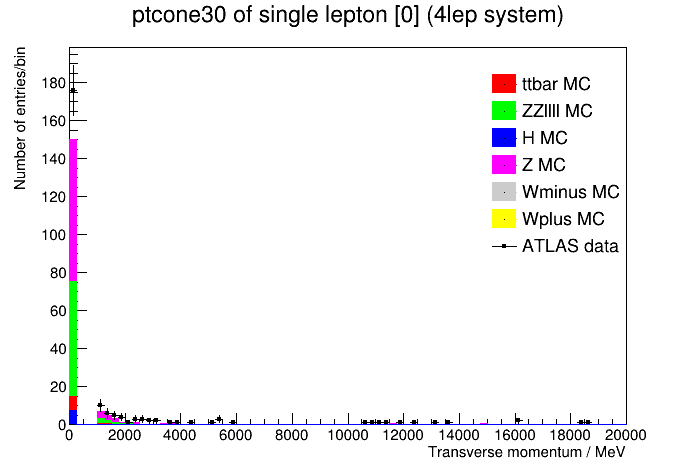
\includegraphics[width=\linewidth]{plots/06-03-2021/07-28_06-03-21.png}
        (A)
    \end{minipage}\hfill
    \begin{minipage}{0.5\textwidth}
        \centering
        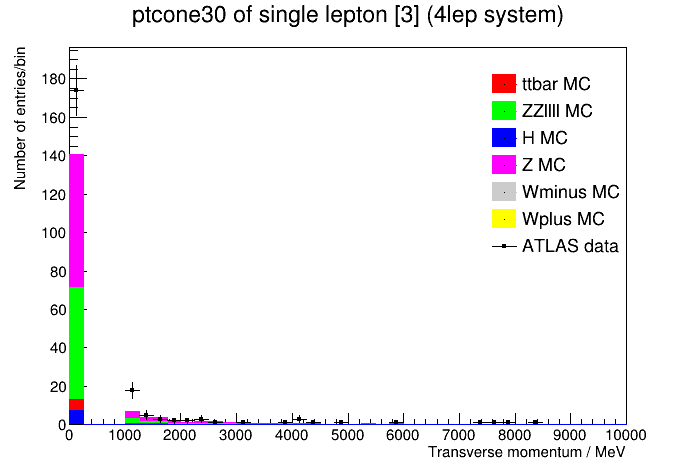
\includegraphics[width=\linewidth]{plots/06-03-2021/08-26_06-03-21.png}
        (B)
    \end{minipage}
    \caption{(A) ptcone of lepton [0] (B) ptcone of lepton [3]}
    \label{fig:07-28_06-03-21}
\end{figure}

\begin{figure}[h!]
    \centering
    \begin{minipage}{0.5\textwidth}
        \centering
        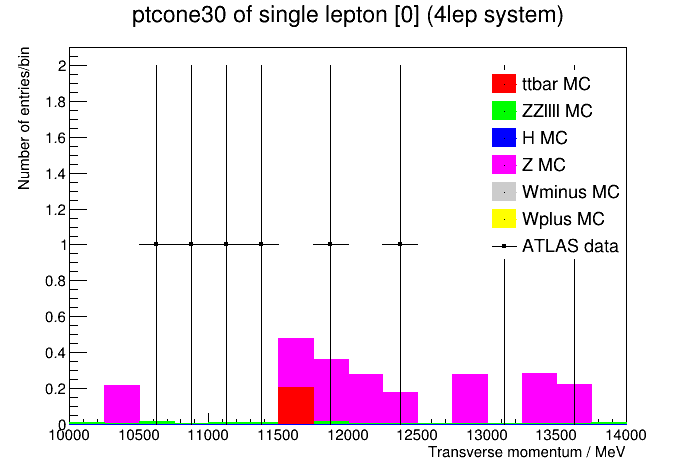
\includegraphics[width=\linewidth]{plots/06-03-2021/07-29_06-03-21.png}
        (A)
    \end{minipage}\hfill
    \begin{minipage}{0.5\textwidth}
        \centering
        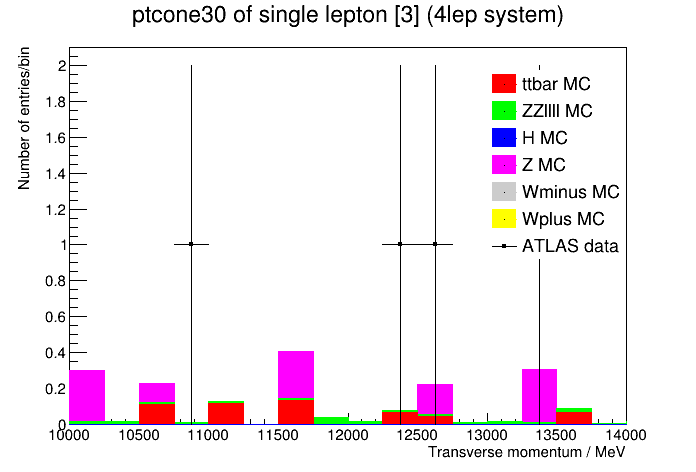
\includegraphics[width=\linewidth]{plots/06-03-2021/08-28_06-03-21.png}
        (B)
    \end{minipage}
    \caption{(A) ptcone30 of lepton [0] (B) ptcone30 of lepton [3]}
    \label{fig:07-29_06-03-21}
\end{figure}

\begin{figure}[h!]
    \centering
    \begin{minipage}{0.5\textwidth}
        \centering
        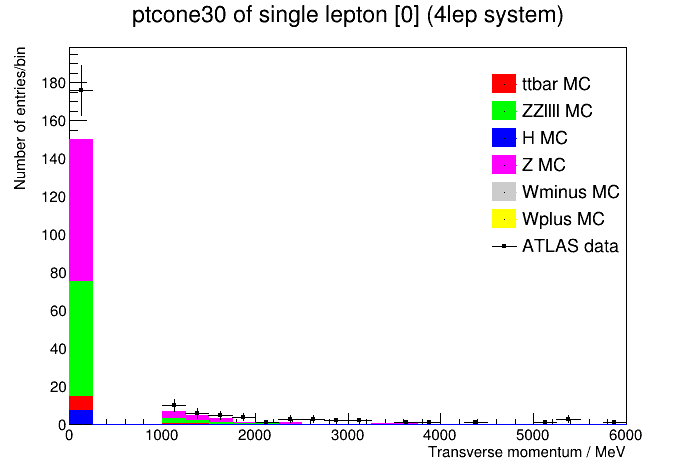
\includegraphics[width=\linewidth]{plots/06-03-2021/07-30_06-03-21.png}
        (A)
    \end{minipage}\hfill
    \begin{minipage}{0.5\textwidth}
        \centering
        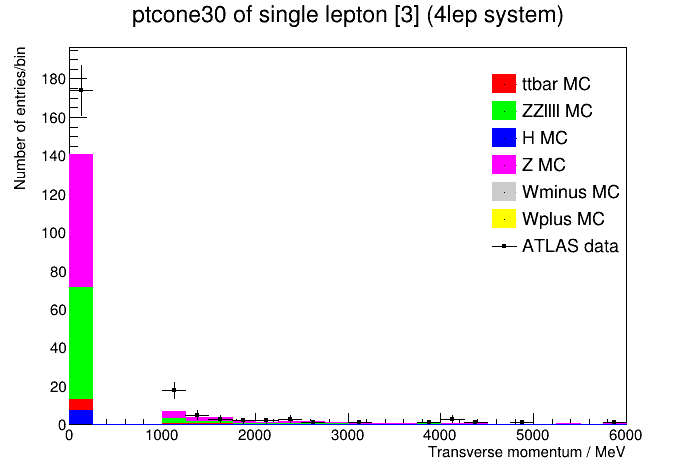
\includegraphics[width=\linewidth]{plots/06-03-2021/08-29_06-03-21.png}
        (B)
    \end{minipage}
    \caption{(A) ptcone30 of lepton [0] (B) ptcone30 of lepton [3]}
    \label{fig:07-30_06-03-21}
\end{figure}

\begin{figure}[h!]
    \centering
    \begin{minipage}{0.5\textwidth}
        \centering
        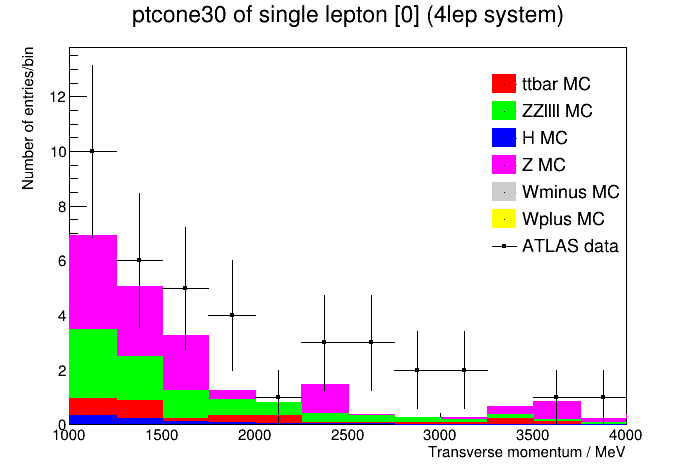
\includegraphics[width=\linewidth]{plots/06-03-2021/07-32_06-03-21.png}
        (A)
    \end{minipage}\hfill
    \begin{minipage}{0.5\textwidth}
        \centering
        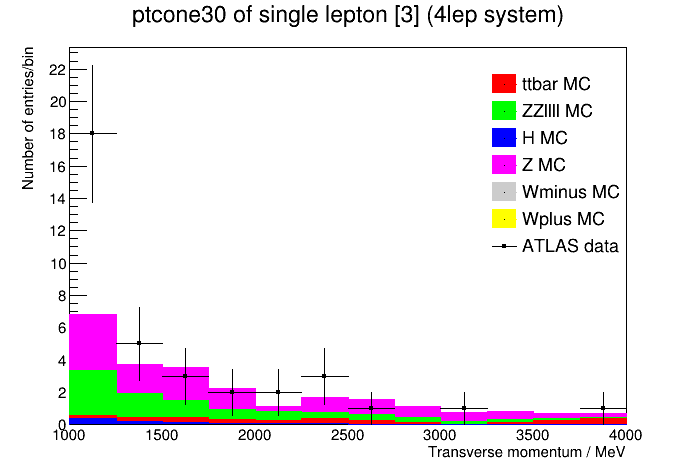
\includegraphics[width=\linewidth]{plots/06-03-2021/08-31_06-03-21.png}
        (B)
    \end{minipage}
    \caption{(A) ptcone30 of lepton [0] (B) ptcone30 of lepton [3])}
    \label{fig:07-32_06-03-21}
\end{figure}

\begin{figure}[h!]
    \centering
    \begin{minipage}{0.5\textwidth}
        \centering
        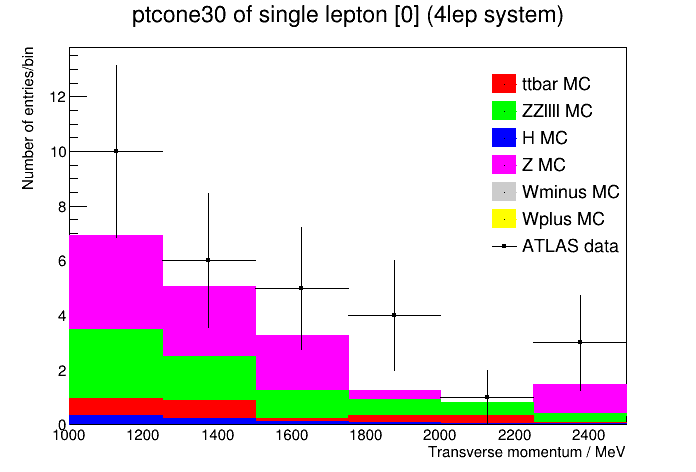
\includegraphics[width=\linewidth]{plots/06-03-2021/07-34_06-03-21.png}
        (A)
    \end{minipage}\hfill
    \begin{minipage}{0.5\textwidth}
        \centering
        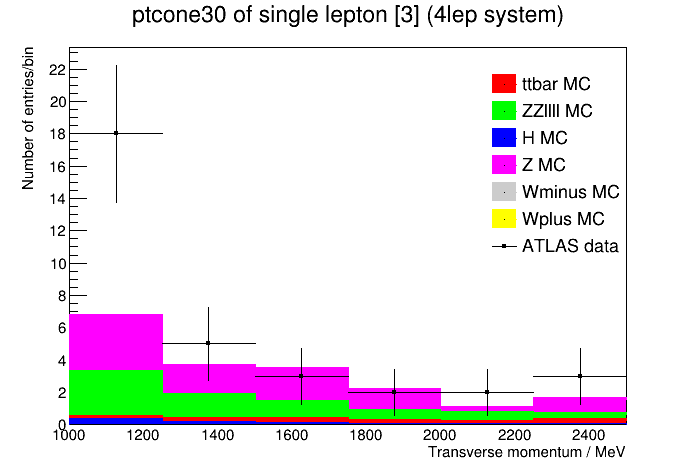
\includegraphics[width=\linewidth]{plots/06-03-2021/08-33_06-03-21.png}
        (B)
    \end{minipage}
    \caption{(A) ptcone30 of lepton [0] (B) ptcone30 of lepton [3]}
    \label{fig:07-33_06-03-21}
\end{figure}

%%%%%%%%%%%%% 10:00 %%%%%%%%%%%%%
\subsubsection{10:00 - ETCone20 of single lepton [3] (Higgs)}
Plotting the etcone20 of lepton [3].
\\
Cuts used in Fig.\ref{}:
\begin{lstlisting}
lepCut ="(" + "lep_n==4" + "&&" + t_c_cut + "&&" + lep_pair_inv_mass_cut + "&&" + invar_mass_cut +  ")"
\end{lstlisting}

\begin{figure}[h!]
    \centering
    \begin{minipage}{0.5\textwidth}
        \centering
        \includegraphics[width=\linewidth]{plots/06-03-2021/}
        (A)
    \end{minipage}\hfill
    \begin{minipage}{0.5\textwidth}
        \centering
        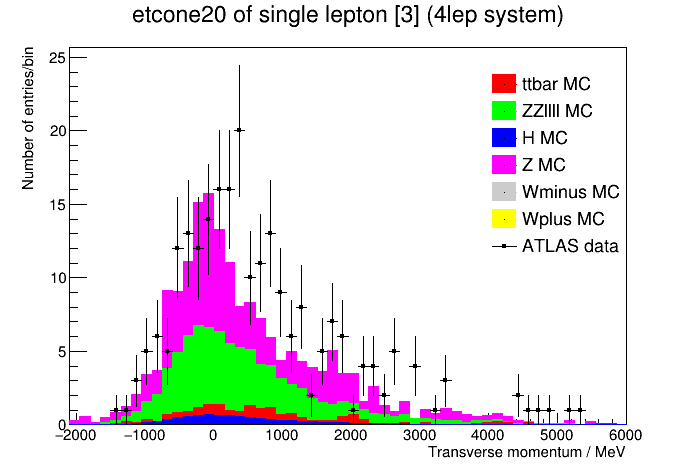
\includegraphics[width=\linewidth]{plots/06-03-2021/10-02_06-03-21_.png}
        (B)
    \end{minipage}
    \caption{(A)  (B) ETCone20 of single lepton [3]}
    \label{fig:10-00_}
\end{figure}

%%%%%%%%%%%%% 14:00 %%%%%%%%%%%%% - Invar-mass of 4 lep for Hiigs with invar-mass cuts, lepton cobination cuts, PT cuts, ETCone cuts, PTCone cuts
\subsubsection{14:00 - Invariant mass of 4 lep with all cuts so far (Higgs)}
Plotting the invariant mass with possible final cuts.
\\
Cuts used in Fig.\ref{fig:14-00_06-03-21}:
\begin{lstlisting}
    # Allowed processes: ee mumu, ee ee, mumu mumu
    # For an allowed process, the sum of charge * type == 0 
    t_c_b = "(lep_charge[{0}] * lep_type[{0}])"  
    t_c = ""
    
    for i in range(4):
        if i != 0:
            t_c += " + "
        t_c += t_c_b.format(i)

    t.SetAlias("t_c_sum", t_c)
    t_c_cut = "t_c_sum == 0"
    
    
    # Generate invariant mass range cut (110 GeV < m_{llll} < 133 GeV)
    invar_mass_cut = "(inv_mass_4 > 110e3 && inv_mass_4 < 133e3)"
    
    # etcone20 (BASIC) cut
    etcone_cut = "( lep_etcone20[0] < 2e3 && lep_etcone20[1] < 2e3 && lep_etcone20[2] < 2e3 && lep_etcone20[3] < 2e3 )"
    
    # etcone (BASIC) cut
    ptcone_cut = "( lep_ptcone30[0] < 2e3 &&  lep_ptcone30[1] < 2e3 && lep_ptcone30[2] < 2e3 &&  lep_ptcone30[3] < 2e3)"
    
    # Transverse Momentum cut
    pt_cut = "( lep_pt[0] < 70e3 && lep_pt[1] < 70e3 &&  lep_pt[2] < 70e3 &&  lep_pt[3] < 70e3)"
    
    # Invariant mass of the two lepton pairs 
    # one pair has to be within the mass width of Z boson.
    # with another which does not (the virtual z boson)
    # Will have mulitple pair cominations so need to calculate invariant mass for all possible combinations (combinatorics)

    lep2_invar_mass_str = "sqrt(2*lep_pt[{0}]*lep_pt[{1}]*(cosh(lep_eta[{0}]-lep_eta[{1}])-cos(lep_phi[{0}]-lep_phi[{1}])))"

    t_c_pair = "(lep_charge[{0}] * lep_type[{0}]) + (lep_charge[{1}] * lep_type[{1}])"

    lep_pair_inv_mass_cut = ""

    i = 0
    for j in range(1, 4):
        for k in range(1, 3):
            for l in range(2, 4):
                if j != k and j != l and k != l and k < l:
                    if not (j == 1 and k == 2 and l == 3):
                        lep_pair_inv_mass_cut += " || "
                    lep_pair_inv_mass_cut += lep2_invar_mass_str.format(i, j) + " > 60e3 && " + lep2_invar_mass_str.format(i, j) + " < 150e3 && " + lep2_invar_mass_str.format(k,l) + " < 60e3" + " && " + t_c_pair.format(i, j) + " == 0 && " + t_c_pair.format(k,l) + " == 0" + " || " + lep2_invar_mass_str.format(k, l) + " > 60e3 && " + lep2_invar_mass_str.format(k, l) + " < 150e3 && " + lep2_invar_mass_str.format(i,j) + " < 60e3" + " && " + t_c_pair.format(k, l) + " == 0 && " + t_c_pair.format(i, j) + " == 0"
    
    # Calulcate invariant mass of Higgs from the 4 leptons.
    x = "2 * lep_pt[{0}] * lep_pt[{1}]*(cosh(lep_eta[{0}]-lep_eta[{1}]) - cos(lep_phi[{0}]-lep_phi[{1}]))"
    s = ""

    for i in range(4):
        for j in range(i+1, 4):
            if not (i == 0 and j == 1):
                s += "+"
            s += x.format(i, j)
 
    t.SetAlias("s", s)
    t.SetAlias("inv_mass_4", "sqrt(s)")

    lepCut ="(" + "lep_n==4" + "&&" + t_c_cut + "&&" + lep_pair_inv_mass_cut + "&&" + invar_mass_cut +  "&&" + etcone_cut + "&&" + ptcone_cut + "&&" + pt_cut + ")"
    
    t.Draw("inv_mass_4 >> h_lep_invar_mass(70,110e3,135e3)", weighting + "*" + lepCut)
\end{lstlisting}

\begin{figure}[h!]
    \centering
    \begin{minipage}{0.5\textwidth}
        \centering
        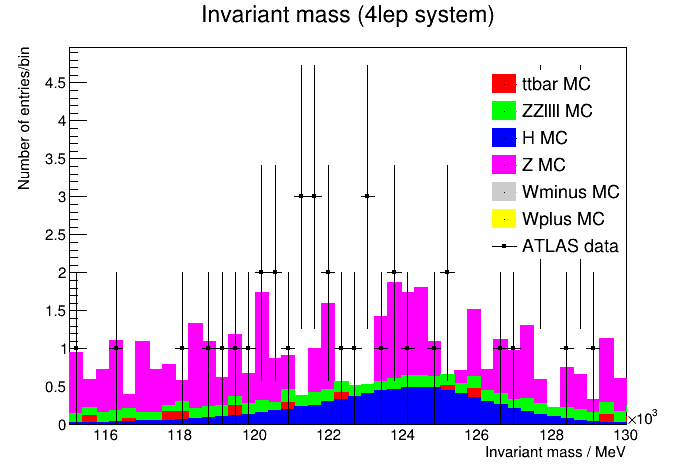
\includegraphics[width=\linewidth]{plots/06-03-2021/14-00_06-03-21.png}
        (A)
    \end{minipage}\hfill
    \begin{minipage}{0.5\textwidth}
        \centering
        \includegraphics[width=\linewidth]{plots/06-03-2021/}
        (B)
    \end{minipage}
    \caption{(A) Invariant mass of the 4 lepton system looking for Higgs candidates. (B) Invariant mass of the 4 lepton system looking for Higgs candidates log-y plot.  Cuts: possibly final (see cuts 14:00 06/03/21)}
    \label{fig:14-00_06-03-21}
\end{figure}

%%%%%%%%%%%%% 15:28 %%%%%%%%%%%%%
\subsubsection{16:26 - Cross section of Higgs with cuts so far}
Cross section:
\\
$9.541 \pm 7.697 \pm 3.944 \pm 0.016 \text{ fb}$

%%%%%%%%%%%%% 15:26 %%%%%%%%%%%%%
\subsubsection{16:26 - Vary Invariant mass cut to estimate syst. uncertainty (Higgs)}
Cross section:
\\
$\sigma(H \rightarrow Z Z^{(*)} \rightarrow llll) = 9.541 \pm 7.697 \pm 3.944 \pm 0.016 \text{ fb}$

\subsubsection{16:30 - End day}
If had more time, would apply the same analysis as for Z where each cut is varied independently to give a systematic uncertainty for each cut and then add the uncertainties together in quadrature.

%%%%%%%%%%%%%%%%%%%%%%%%%%%%%%%%%%%%%%%%%%%%%%%%%%%%%%%%%%%%%%%%%%%%%%%%%%%%%%%%%%%%%%%%%%%%%%%%%%%%%%%%%%%%%%%%%%%%%%%%%%%%%%%%%%%%%%%%%%%%%%%%%%%%%%%%%%%%%%%%%%%%%%%%%%%%%%%%%%%%%%%%%%%%%%%%%%%%%%%%%%%%%%%%%%%%%%%%%%%%%%%%%%%%%%%%%%%%%%%%%%%%%%%%%%%%%%%%%%%%%%%%%%%%%%%%%%%%%%%%%%%%%%%%%%%%%%%%%%%%%%%%%%%%%%%%%%%%%%%%%%%%%%%%%%%%%%%%%%%%%%%%%%%%%%%%%%%%%%%%%%%%%%%%%%%%%%%%%%%%%%%%%%%%%%%%%%%%%%%%%%%%%%%%%%%%%%%%%%%%%%%%%%%%%%%%%%%%%%%%%%%%%%%%%%%%%%%%%%%%%%%%%%%%%%%%%%%%%%%%
% \begin{figure}[h!]
%     \centering
%     \begin{minipage}{0.5\textwidth}
%         \centering
%         \includegraphics[width=\linewidth]{plots/06-03-2021/}
%         (A)
%     \end{minipage}\hfill
%     \begin{minipage}{0.5\textwidth}
%         \centering
%         \includegraphics[width=\linewidth]{plots/06-03-2021/}
%         (B)
%     \end{minipage}
%     \caption{(A)  (B)}
%     \label{}
% \end{figure}
